\chapter{Meetings with external resources}

\section{Meetings with supervisor}
The team had meetings with the supervisor every other week throughout the project, except for the period when the team was absent for the school trip to China. After this period, the semester was ended, and all meetings after this point was initiated exclusively by the team. All these meetings were held in the break room area outside the supervisor's office.

\begin{table}[H]
\centering
\begin{tabular}{|l|l|p{12.6cm}|}
\hline
\textbf{Week \#} & \textbf{Date}&\textbf{Summary}\\\hline
5& 31.01&Get familiar with supervisor's tasks and what we were to write in the different project documents requested by the subject administration.\\\hline
7 &14.02&Feedback on report, tips on how we could improve our risk analysis and guidance on how to approach customer if he does not provide us with necessary information.\\\hline
9 &27.02& Feedback and questions on mid-term report.\\\hline
11 &14.03& Feedback on report, especially regarding requirement specification and how we should represent the development process in the report.\\\hline
13 &03.04&General feedback on report and status update before the team left for China.\\\hline
19&&\\\hline
\end{tabular}
\caption{Overview on meetings with supervisor}
\end{table}

\section{Meetings with customer}
These meetings were held in the room on NTNU that was provided by the subject's administration. Initially, they were held every week, until the customer said he did not feel it was necessary to have these meetings that often. This was later withdrawn, and we went back to our original agreement.
\begin{table}[H]
\centering
\begin{tabular}{|l|p{14.7cm}|}
\hline
\textbf{Date}&\textbf{Summary}\\\hline
24.01& Introductory meeting with customer. Team and customer got to know each other. Assignment presented and discussed. Customer wanted team to brainstorm to figure out what should be in the app.\\\hline
31.01& Team introduced the concepts they reached after brainstorming. Also discussed existing solutions and possible architectual solutions for the app.\\\hline
07.02& Discussed back-end solutions. Clarifications regarding documentation and information about the customer's research program.\\\hline
14.02& Team suggested deadline for changes in requirement specification, approved by customer. Discussed architecture, whether GUI should be vertical and/or horizontal and also if we only should focus on developing the application for mobile phones.\\\hline
21.02&Demonstration of prototype. Customer approved the requirement specification, but had some feedback on the prototype that led to some changes and additions in the specification. Discussed possible hardware solutions and what the team were to focus on for the next iteration. \\\hline
%28.02 kunde følte ikke det var nødvendig med møte
%07.03 kunde bortreist
14.03& Customer reviewed the app. Approved of the name the team came up with for the app. Wanted to use the meetings on Fridays as a sprint meeting, review the requirement specification and make a list of what we should prioritize in the following sprint.\\\hline
%21.03 glemte møteinnkalling
28.03& Demonstration and review of the app.\\\hline
02.04& Last meeting with customer before team left for China. Customer wants to do usability testing with his co-workers at SINTEF. Requests that we apply textual descriptions on sites that are not completely finished.\\\hline
%09.04 Kina
%16.04 Påske
%25.04 prøvde å få kontakt med kunde
02.05& Demonstration and review of the app. Updated Kanban-board. Customer emphasized that the team should provide a thourough description of further development in the report. \\\hline
\end{tabular}
\caption{Overview on meetings with customer}
\end{table}







\chapter{Example of project documents}


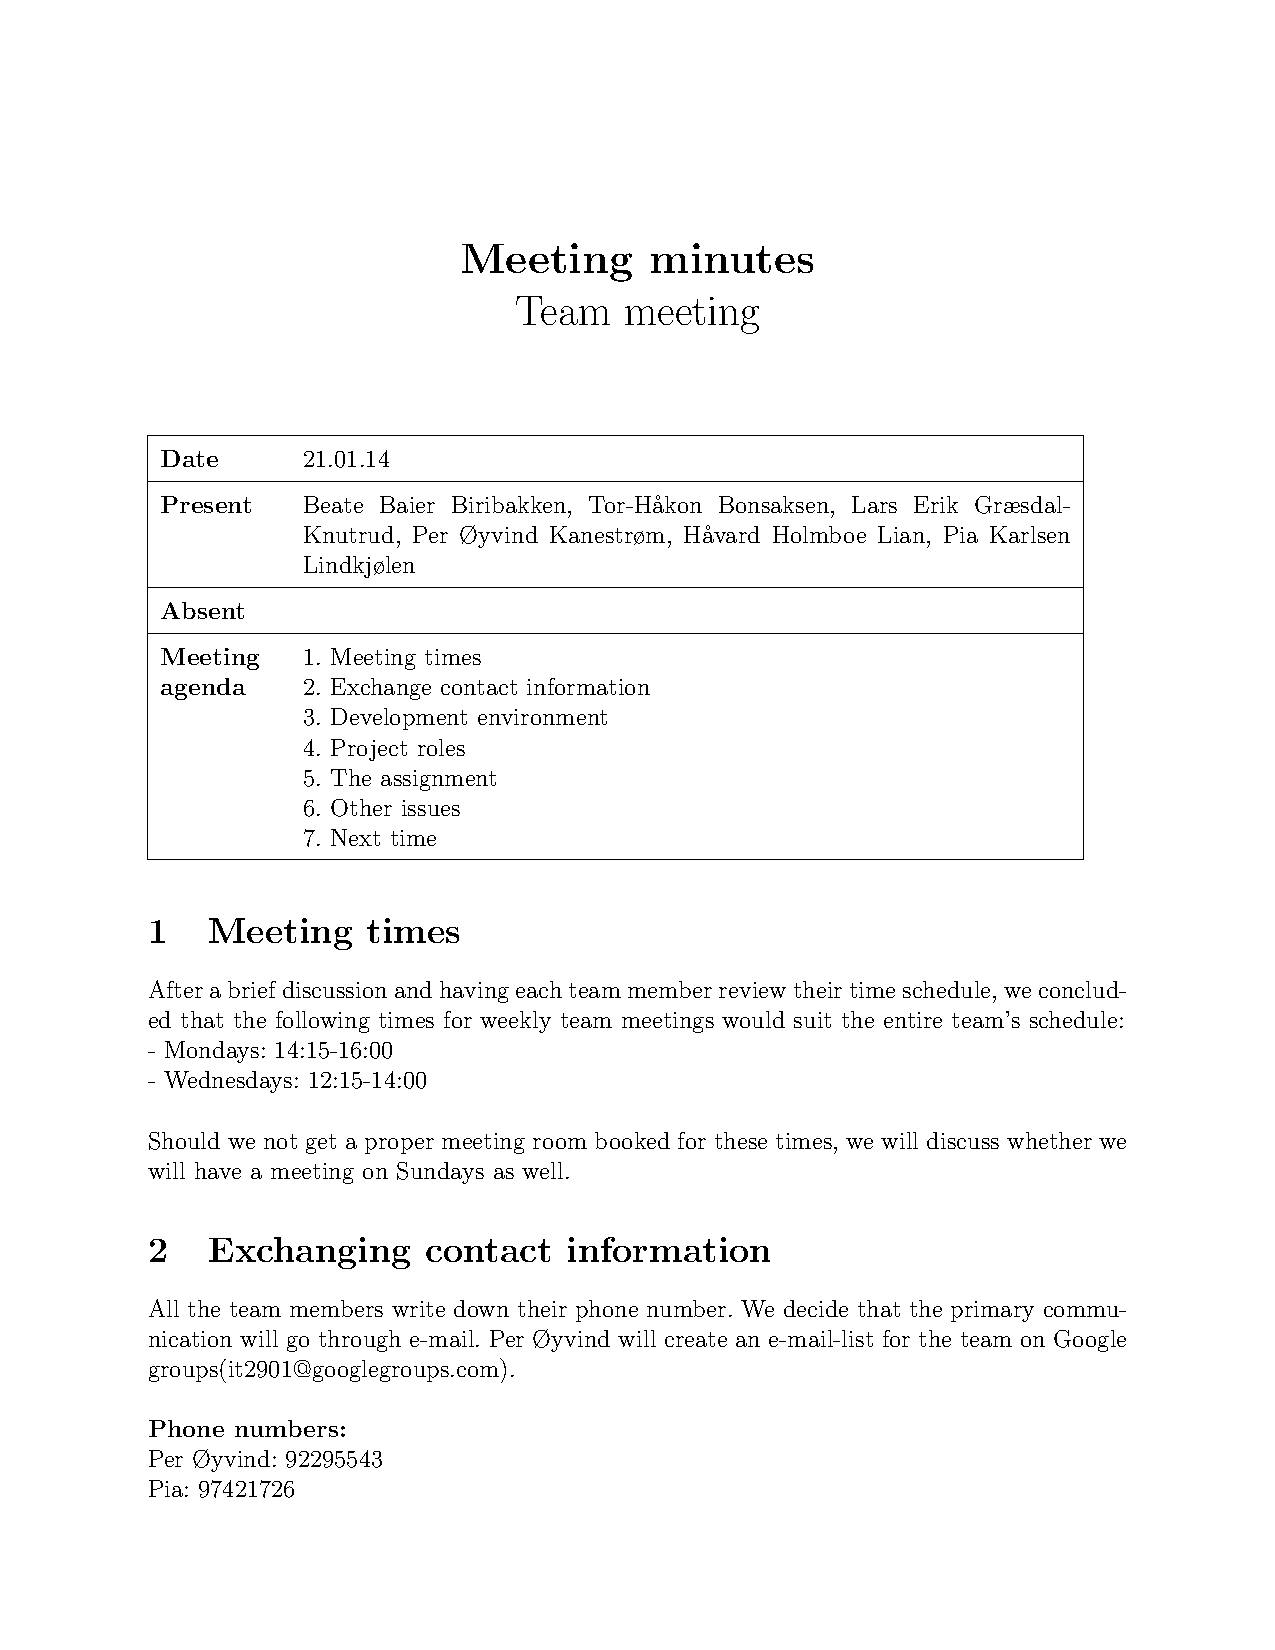
\includepdf[pages=1,pagecommand=\section{Meeting report example}, frame=true, scale=0.76, trim=0mm 10mm 0mm 20mm, clip]{appendix/meetings/firstteammeeting.pdf}
\includepdf[pages=2-3, pagecommand={},fitpaper=true, frame=true, scale=0.76]{appendix/meetings/firstteammeeting.pdf}


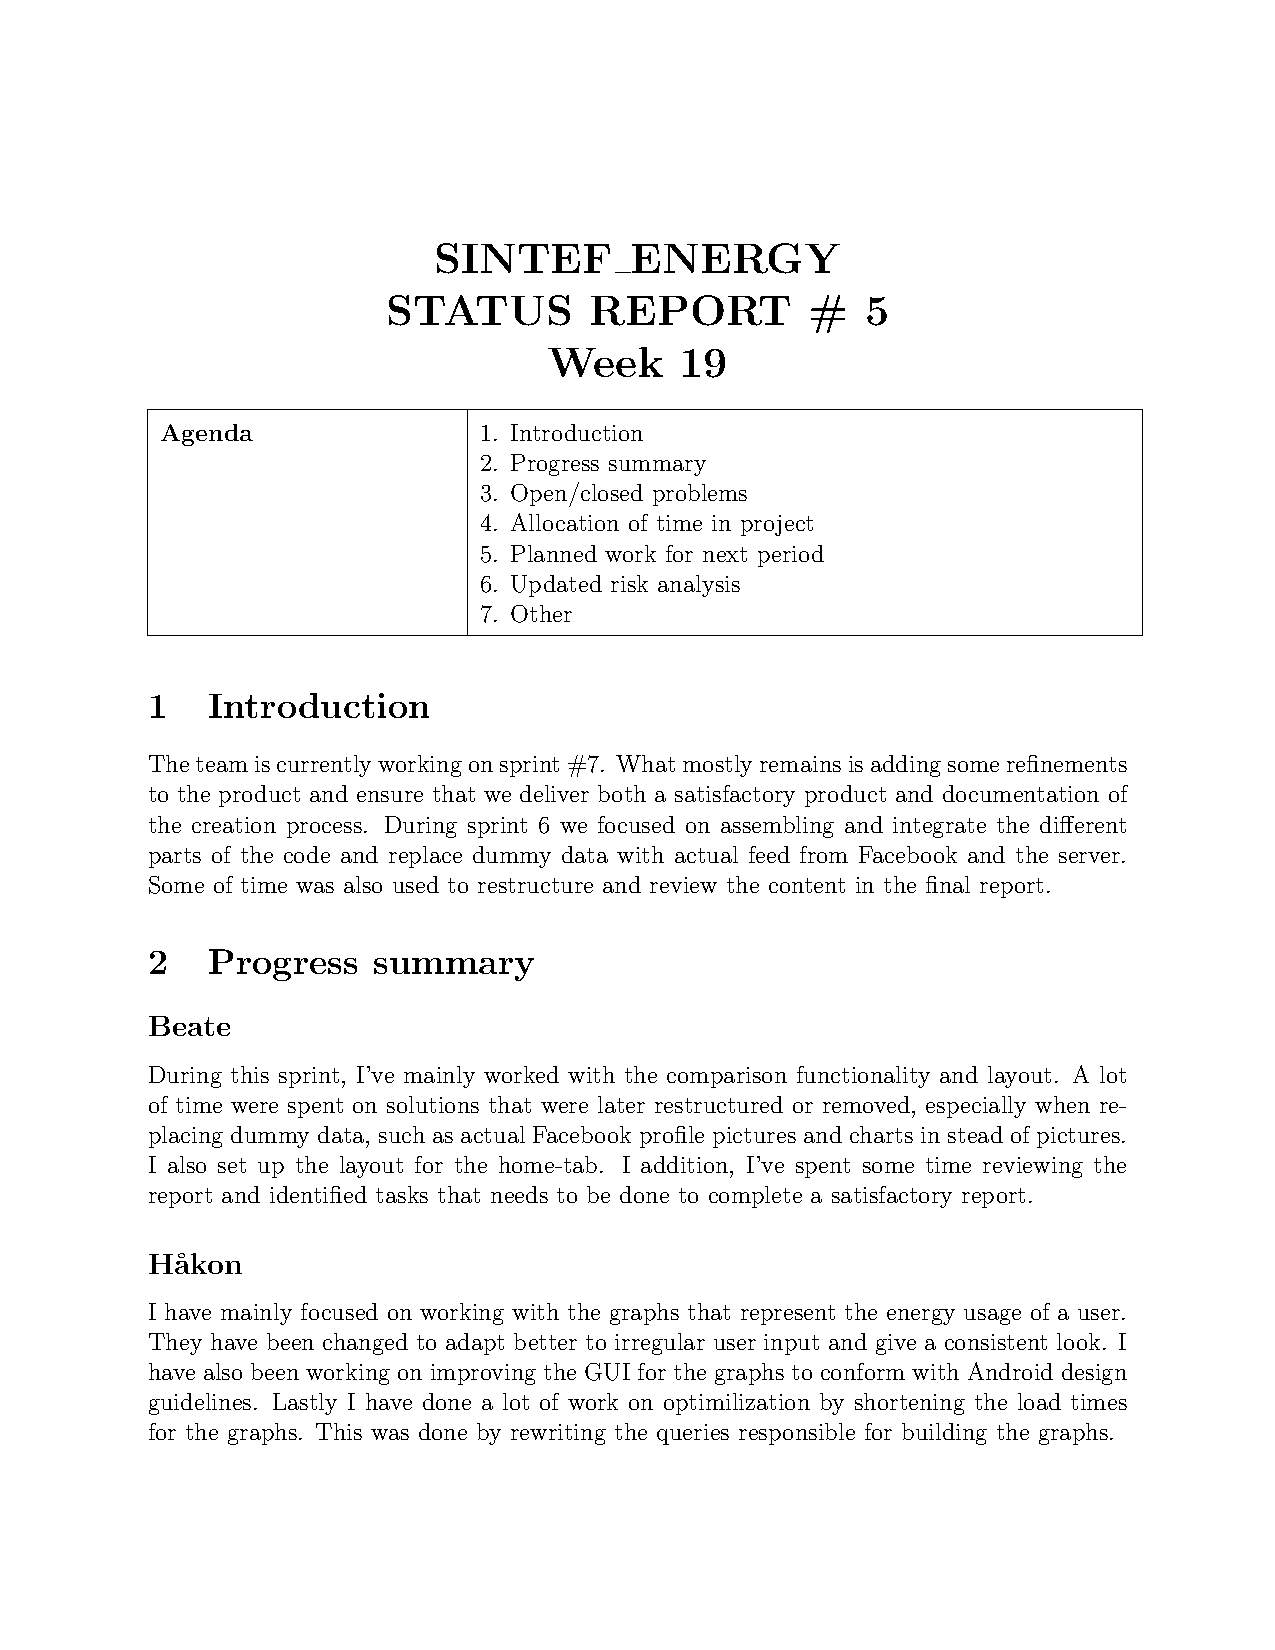
\includepdf[pages=1,pagecommand=\section{Status report example}, frame=true, scale=0.76, trim=0mm 20mm 0mm 20mm, clip]{appendix/meetings/supervisor.pdf}

\includepdf[pages=2-3,pagecommand={},fitpaper=true, frame=true, scale=0.76]{appendix/meetings/supervisor.pdf}
